\begin{center}
    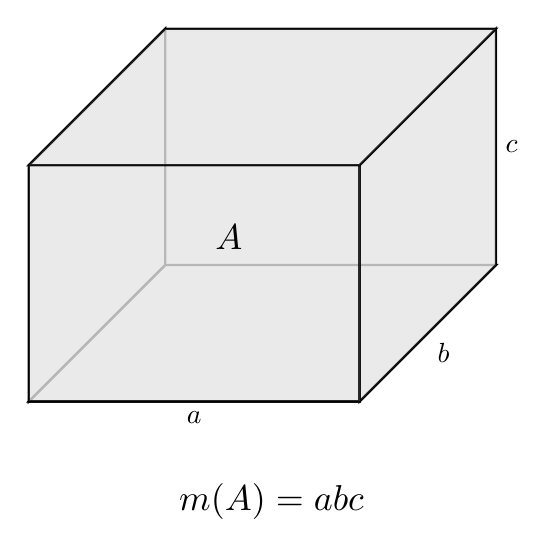
\begin{tikzpicture}[scale=1.5]
        \pgfmathsetmacro{\Depth}{2.8}
        \pgfmathsetmacro{\Height}{3}
        \pgfmathsetmacro{\Width}{2}
        \coordinate (O) at (0,0,0);
        \coordinate (A) at (0,\Width,0);
        \coordinate (B) at (0,\Width,\Height);
        \coordinate (C) at (0,0,\Height);
        \coordinate (D) at (\Depth,0,0);
        \coordinate (E) at (\Depth,\Width,0);
        \coordinate (F) at (\Depth,\Width,\Height);
        \coordinate (G) at (\Depth,0,\Height);

        \draw[black,thick] (O) -- (C) -- (G) -- (D) -- cycle;% Bottom Face
        \draw[black,thick] (O) -- (A) -- (E) -- (D) -- cycle;% Back Face
        \draw[black,thick] (O) -- (A) -- (B) -- (C) -- cycle;% Left Face
        \draw[black,thick,fill=gray!20,opacity=0.8] (D) -- (E) -- (F) -- (G) -- cycle;% Right Face
        \draw[black,thick,fill=gray!20,opacity=0.8] (C) -- (B) -- (F) -- (G) -- cycle;% Front Face
        \draw[black,thick,fill=gray!20,opacity=0.8] (A) -- (B) -- (F) -- (E) -- cycle;% Top Face

        %% Following is for debugging purposes so you can see where the points are
        %% These are last so that they show up on top
        % \foreach \xy in {O, A, B, C, D, E, F, G}{
        %    \node at (\xy) {\xy};
        % }

        \path (C) -- node[below] {\(a\)} (G)
        -- node[below right] {\(b\)} (D)
        -- node[right] {\(c\)} (E);

        \node[scale=1.3] at (1, 0.7, 1.2) {\(A\)};

        \node[scale=1.3] at (0.9, -2) {\(m(A) = abc\)};
    \end{tikzpicture}
\end{center}

\section*{Construction of Measure}

이제 본격적으로 집합을 재보도록 하겠습니다. 우리가 잴 수 있는 집합들부터 시작합니다. \(\R^p\)에서 논의할 건데, 이제 여기서부터는 \(\R\)의 구간의 열림/닫힘을 모두 포괄하여 정의합니다. 즉, \(\R\)의 구간이라고 하면 \([a, b], (a, b), [a, b), (a, b]\) 네 가지 경우를 모두 포함합니다.

\defn. \note{\(\R^p\)의 구간} \(a_i, b_i \in \R\), \(a_i \leq b_i\) 라 하자. \(I_i\)가 \(\R\)의 구간이라고 할 때, \(\R^p\)의 구간은
\[
    \prod_{i=1}^p I_i = I_1 \times \cdots \times I_p,
\]
와 같이 정의한다.

예를 들어 \(\R^2\)의 구간이라 하면 직사각형 영역, \(\R^3\)의 구간이라 하면 직육면체 영역을 떠올릴 수 있습니다. 단, 경계는 포함되지 않을 수도 있습니다.

이러한 구간들을 유한개 모아 합집합하여 얻은 집합을 모아 elementary set이라 합니다.

\defn. \note{Elementary Set} 어떤 집합이 유한개 구간의 합집합으로 표현되면 그 집합을 elementary set이라고 한다. 그리고 \(\R^p\)의 elementary set의 모임을 \(\Sigma\)로 표기한다.

임의의 구간은 유계입니다. 따라서 구간의 유한한 합집합도 유계일 것입니다.

\rmk 임의의 elementary set은 유계이다.

Elementary set의 모임에서 집합의 연산을 정의할 수 있을 것입니다. 이 때, \(\Sigma\)가 ring이 된다는 것을 간단하게 확인할 수 있습니다.

\prop. \(\Sigma\)는 ring이다. 하지만 전체 공간인 \(\R^p\)를 포함하고 있지 않기 때문에 \(\sigma\)-ring은 아니다.

구간의 길이를 재는 방법은 아주 잘 알고 있습니다. 유한개 구간의 합집합인 elementary set에서도 쉽게 잴 수 있습니다. 이제 길이 함수 \(m: \Sigma \ra [0, \infty)\) 을 정의하겠습니다. 아직 measure는 아닙니다.

\defn. \(a_i, b_i \in \R\) 가 구간 \(I_i\)의 양 끝점이라 하자. \(\R^p\)의 구간 \(I = \ds \prod_{i=1}^p I_i\) 에 대하여,
\[
    m(I) = \prod_{i=1}^p (b_i - a_i)
\]
로 정의한다.

\defn. \(I_i\)가 쌍마다 서로소인 \(\R^p\)의 구간이라 하자. \(A = \ds\bigcup_{i=1}^n I_i\) 에 대하여
\[
    m(A) = \sum_{i=1}^n m(I_i)
\]
로 정의한다.

\(\R, \R^2, \R^3\)에서 생각해보면 \(m\)은 곧 길이, 넓이, 부피와 대응되는 함수임을 알 수 있습니다. 또한 쌍마다 서로소인 구간의 합집합에 대해서는 각 구간의 함숫값을 더한 것으로 정의합니다. 어떤 집합을 겹치지 않게 구간으로 나눌 수 있다면, 집합의 `길이'가 각 구간의 `길이' 합이 되는 것은 자연스럽습니다.

그리고 이 정의는 well-defined 입니다. \(A \in \Sigma\) 에 대해서 서로소인 유한개 구간의 합집합으로 나타내는 방법이 유일하지 않아도, \(m\) 값은 같습니다.

\rmk \(m\)은 \(\Sigma\) 위에서 additive이다. 따라서 \(m : \Sigma \ra [0, \infty)\) 은 additive set function이다.

여기서 추가로 regularity 조건을 만족했으면 좋겠습니다.

\defn. \note{Regularity} Set function \(\mu: \Sigma \ra [0, \infty]\) 가 additive라 하자. 모든 \(A \in \Sigma\) 와 \(\epsilon > 0\) 에 대하여
\begin{center}
    닫힌집합 \(F \in \Sigma\), 열린집합 \(G \in \Sigma\) 가 존재하여 \(F \subset A \subset G\) 이고 \(\mu(G) - \epsilon \leq \mu(A) \leq \mu(F) + \epsilon\)
\end{center}
이면 \(\mu\)가 \(\Sigma\) 위에서 \textbf{regular}하다고 정의한다.

위에서 정의한 \(m\)이 regular한 것은 쉽게 확인할 수 있습니다.

이제 set function \(\mu: \Sigma \ra [0, \infty)\) 가 finite, regular, additive 하다고 가정합니다.

\defn. \note{Outer Measure} \(E \in \mc{P}(\R^p)\) 의 \textbf{outer measure} \(\mu^\ast: \mc{P}(\R^p) \ra [0, \infty]\) 는
\[
    \mu^\ast(E) = \inf \left\{\sum_{n=1}^\infty \mu(A_n) : \text{열린집합 } A_n \in \Sigma \text{ 에 대하여 } E \subset \bigcup_{n=1}^\infty A_n\right\}.
\]
로 정의한다.

Outer measure라 부르는 이유는 \(E\)의 바깥에서 길이를 재서 근사하기 때문입니다. Outer measure는 모든 power set에 대해서 정의할 수 있으니, 이를 이용해서 모든 집합을 잴 수 있으면 좋겠습니다. 하지만 measure가 되려면 countably additive 해야하는데, 이 조건이 가장 만족하기 까다로운 조건입니다. 실제로 countably additive 조건이 성립하지 않습니다.

\rmk
\begin{itemize}
    \item \(\mu^\ast \geq 0\) 이다.
    \item \(E_1 \subset E_2\) 이면 \(\mu^\ast(E_1) \leq \mu^\ast(E_2)\) 이다. (단조성)
\end{itemize}

\thm{11.8}
\begin{enumerate}
    \item \(A \in \Sigma\) 이면 \(\mu^\ast(A) = \mu(A)\).\footnote{\(A\)가 open이 아니면 자명하지 않은 명제입니다.}
    \item Countable subadditivity가 성립한다.
          \[
              \mu^\ast\paren{\bigcup_{n=1}^\infty E_n} \leq \sum_{n=1}^\infty \mu^\ast(E_n), \quad (\forall E_n \in \mc{P}(\R^p))
          \]
\end{enumerate}

\pf \\
(1) \(A \in \Sigma\), \(\epsilon > 0\) 라 두자. \(\mu\)의 regularity를 이용하면, 열린집합 \(G \in \Sigma\) 가 존재하여 \(A \subset G\) 이고
\[
    \mu^\ast(A) \leq \mu(G) \leq \mu(A) + \epsilon
\]
이다. \(\mu^\ast\)의 정의에 의해 열린집합 \(A_n \in \Sigma\) 가 존재하여 \(A \subset \ds \bigcup_{n=1}^\infty A_n\) 이고
\[
    \sum_{n=1}^\infty \mu(A_n) \leq \mu^\ast(A) + \epsilon
\]
이다. 마찬가지로 regularity에 의해 닫힌집합 \(F \in \Sigma\) 가 존재하여 \(F\subset A\) 이고 \(\mu(A) \leq \mu(F) + \epsilon\) 이다. \(F \subset \R^p\) 는 유계이고 닫힌집합이므로 compact set이고, finite open cover를 택할 수 있다.
\begin{center}
    적당한 \(N \in \N\) 에 대하여 \(F \subset \ds\bigcup_{i=1}^N A_{i}\) 가 성립한다.
\end{center}
따라서
\[
    \mu(A) \leq \mu(F) + \epsilon \leq \sum_{i=1}^N \mu(A_i) \leq \sum_{i=1}^n \mu(A_i) + \epsilon \leq \mu^\ast(A) + 2\epsilon
\]
이제 \(\epsilon \ra 0\) 로 두면 \(\mu(A) = \mu^\ast(A)\) 를 얻는다.

(2) 부등식의 양변이 모두 \(\infty\) 이면 증명할 것이 없으므로, 양변이 모두 유한하다고 가정하여 모든 \(n\in \N\) 에 대해 \(\mu^\ast(E_n) < \infty\) 라 하자. \(\epsilon > 0\) 로 두고, 각 \(n \in \N\) 에 대하여 열린집합 \(A_{n, k} \in \Sigma\) 가 존재하여
\begin{center}
    \(E_n \subset \ds \bigcup_{k=1}^\infty A_{n, k}\) 이고 \(\ds \sum_{k=1}^\infty \mu(A_{n,k}) \leq \mu^\ast(E_n) + 2^{-n}\epsilon\) 이다.
\end{center}
\(\mu^\ast\)는 하한(infimum)으로 정의되었기 때문에,
\[
    \mu^\ast\paren{\bigcup_{n=1}^\infty E_n} \leq \sum_{n=1}^\infty \sum_{k=1}^\infty \mu(A_{n,k}) \leq \sum_{n=1}^\infty \mu^\ast(E_n) + \epsilon
\]
가 성립하고, \(\epsilon \ra 0\) 로 두면 부등식이 성립함을 알 수 있다.

\dots

Countably additive 조건이 성립하는 집합들만 모아서 measure를 construct 하려고 합니다. 아래 내용은 이를 위한 사전 준비 작업입니다.

\notation \note{대칭차집합} \(A \symd B = (A\bs B) \cup (B \bs A)\).

\defn.
\begin{itemize}
    \item \(d(A, B) = \mu^\ast(A \symd B)\) 로 정의한다.
    \item 집합열 \(A_n\)에 대하여 \(d(A_n, A) \ra 0\) 이면 \(A_n \ra A\) 로 정의한다.
\end{itemize}

\rmk
\begin{itemize}
    \item \(A, B, C \in \R^p\) 에 대하여 \(d(A, B) \leq d(A, C) + d(C, B)\) 이다.
    \item \(A_1, B_2, B_1, B_2 \in \R^p\) 일 때, 다음이 성립한다.
          \[
              \left.\begin{array}{c}d(A_1 \cup A_2, B_1 \cup B_2) \\d(A_1 \cap A_2, B_1 \cap B_2) \\d(A_1 \bs A_2, B_1 \bs B_2)\end{array}\right\}
              \leq d(A_1, B_1) + d(A_2, B_2).
          \]
\end{itemize}

\defn. \note{Finitely \(\mu\)-measurable} 집합 \(A_n \in \Sigma\) 이 존재하여 \(A_n \ra A\) 이면 \(A\)가 \textbf{finitely \(\mu\)-measurable}이라 한다. 그리고 finitely \(\mu\)-measurable한 집합의 모임을 \(\mf{M}_F(\mu)\)로 표기한다.

위 정의는 \(\mu\)라는 set function에 의해 \(\mu^\ast (A_n \symd A) \ra 0\) 이 되는 elementary set \(A_n\)이 존재한다는 의미입니다.

\defn. \note{\(\mu\)-measurable} \(A_n \in \mf{M}_F(\mu)\) 에 대하여 \(A = \ds \bigcup_{n=1}^\infty A_n\) 이면 \(A\)가 \textbf{\(\mu\)-measurable}이라 한다. 그리고 \(\mu\)-measurable한 집합의 모임을 \(\mf{M}(\mu)\)로 표기한다.

\rmk \(\mu^\ast(A) = d(A, \varnothing) \leq d(A, B) + \mu^\ast(B)\).

\prop. \(\mu^\ast(A)\) 또는 \(\mu^\ast(B)\)가 유한하면, 다음이 성립한다.
\[
    \abs{\mu^\ast(A) - \mu^\ast(B)} \leq d(A, B).
\]

\cor \(A \in \mf{M}_F(\mu)\) 이면 \(\mu^\ast(A) < \infty\) 이다.

\pf \(A_n \in \Sigma\) 가 존재하여 \(A_n \ra A\) 이고, \(N \in \N\) 이 존재하여
\[
    \mu^\ast(A) \leq d(A_N, A) + \mu^\ast(A_N) \leq 1 + \mu^\ast(A_N) < \infty
\]
이다.

\cor \(A_n \ra A\) 이고 \(A_n, A \in \mf{M}_F(\mu)\) 이면 \(\mu^\ast(A_n)\ra \mu^\ast(A) < \infty\) 이다.

\pf \(\mu^\ast(A)\), \(\mu^\ast(A_n)\)가 유한하므로, \(n \ra \infty\) 일 때 \(\abs{\mu^\ast(A_n) - \mu^\ast(A)} \leq d(A_n, A) \ra 0\) 이다.

\dots

준비가 끝났으니 measure를 construct 해보겠습니다! \(\mc{P}(\R^p)\)에서는 할 수 없지만 정의역을 \(\mf{M}(\mu)\)로 조금 좁히면 measure가 된다는 뜻입니다.

\thm{11.10} \(\mf{M}(\mu)\)는 \(\sigma\)-algebra 이고 \(\mu^\ast\)는 \(\mf{M}(\mu)\)의 measure가 된다.

\pf \(\mf{M}(\mu)\)가 \(\sigma\)-algebra이고 \(\mu^\ast\)가 \(\mf{M}(\mu)\)에서 countably additive임을 보이면 충분하다.

\note{Step 0} \textit{\(\mf{M}_F(\mu)\)는 ring이다.}

\(A, B \in \mf{M}_F(\mu)\) 라 하자. 그러면 \(A_n, B_n \in \Sigma\) 이 존재하여 \(A_n \ra A\), \(B_n \ra B\) 이 된다. 그러면
\[
    \left.\begin{array}{c}d(A_n \cup B_n, A \cup B) \\ d(A_n \cap B_n, A \cap B) \\ d(A_n \bs B_n, A \bs B)\end{array}\right\}
    \leq d(A_n, A) + d(B_n, B) \ra 0
\]
이므로 \(A_n \cup B_n \ra A \cup B, A_n \bs B_n \ra A\bs B\) 이기 때문에 \(\mf{M}_F(\mu)\)는 ring이다.

\note{Step 1} \textit{\(\mu^\ast\)는 \(\mf{M}_F(\mu)\) 위에서 additive이다}.

\(\Sigma\) 위에서는 \(\mu = \mu^\ast\) 이므로, 위 따름정리에 의해
\[
    \begin{matrix}
        \mu(A_n) \ra \mu^\ast(A), & \mu(A_n\cup B_n) \ra \mu^\ast(A\cup B), \\
        \mu(B_n) \ra \mu^\ast(B), & \mu(A_n\cap B_n) \ra \mu^\ast(A\cap B)
    \end{matrix}
\]
가 성립함을 알 수 있다. 일반적으로 \(\mu(A_n) + \mu(B_n) = \mu(A_n \cup B_n) + \mu(A_n \cap B_n)\) 이므로 여기서 \(n \ra \infty\) 로 두면
\[
    \mu^\ast(A) + \mu^\ast(B) = \mu^\ast(A\cup B) + \mu^\ast(A \cap B)
\]
를 얻는다. \(A \cap B = \varnothing\) 라는 조건이 추가되면 \(\mu^\ast\)가 additive임을 알 수 있다.

\note{Step 2} \textit{\(\mf{M}_F(\mu) = \{A \in \mf{M}(\mu) : \mu^\ast(A) < \infty\}\).}\footnote{\(A\)가 \(\mu\)-measurable인데 \(\mu^\ast(A) < \infty\)이면 \(A\)는 finitely \(\mu\)-measurable이다.}

\quad \claim. 쌍마다 서로소인 \(\mf{M}_F(\mu)\)의 원소들을 잡아 이들의 합집합으로 \(A \in \mf{M}(\mu)\) 를 표현할 수 있다.

\quad \pf \(A_n' \in \mf{M}_F(\mu)\) 에 대하여 \(A = \bigcup A_n'\) 로 두자.
\begin{center}
    \(A_1 = A_1'\), \(n \geq 2\) 이면 \(A_n = A_n' \bs (A_1'\cup \cdots \cup A_{n-1}')\)
\end{center}
와 같이 정의하면 \(A_n\)이 쌍마다 서로소이고 \(A_n \in \mf{M}_F(\mu)\) 임을 알 수 있다.

위 사실을 이용하여 \(A_n \in \mf{M}_F(\mu)\) 에 대하여 \(A = \ds \bigcup_{n=1}^\infty A_n\) 로 두자.
\begin{enumerate}
    \item Countable subadditivity에 의해 \(\ds \mu^\ast(A) \leq \sum_{n=1}^{\infty} \mu^\ast (A_n)\) 가 성립한다.
    \item {\sffamily Step 1}에 의해 \(\ds \bigcup_{n=1}^k A_n \subset A\), \(\ds \sum_{n=1}^{k} \mu^\ast(A_n) \leq \mu^\ast(A)\) 이다. \(k \ra \infty\) 로 두면 \(\ds \mu^\ast(A) \geq \sum_{n=1}^\infty \mu^\ast(A_n)\) 임을 알 수 있다.
\end{enumerate}

따라서 \(\ds \mu^\ast(A) = \sum_{n=1}^\infty \mu^\ast(A_n)\) 이다.\footnote{\(A\)가 countable union of sets in \(\mf{M}_F(\mu)\)이므로 \(\mu^\ast\)도 각 set의 \(\mu^\ast\)의 합이 된다.} \footnote{아직 증명이 끝나지 않았습니다. \(A_n\)은 \(\mf{M}(\mu)\)의 원소가 아니라 \(\mf{M}_F(\mu)\)의 원소입니다.}

이제 \(B_n =\ds \bigcup_{k=1}^n A_k\) 로 두자. \(\mu^\ast(A) < \infty\) 를 가정하면 \(\ds \sum_{n=1}^\infty \mu^\ast(A_n)\)의 수렴성에 의해
\begin{center}
    \(\ds d(A, B_n) = \mu^\ast\paren{\bigcup_{k=n+1}^\infty A_k} = \sum_{k=n+1}^{\infty} \mu^\ast(A_i) \ra 0\) as \(n \ra \infty\)
\end{center}
임을 알 수 있다.

\(B_n \in \mf{M}_F(\mu)\) 이므로 \(C_n \in \Sigma\) 를 잡아 각 \(n \in \N\) 에 대하여 \(d(B_n, C_n)\)를 임의로 작게 만들 수 있다. 그러면 \(d(A, C_n) \leq d(A, B_n) + d(B_n, C_n)\) 이므로 충분히 큰 \(n\)에 대하여 \(d(A, C_n)\)도 임의로 작게 만들 수 있다. 따라서 \(C_n \ra A\) 임을 알 수 있고 \(A \in \mf{M}_F(\mu)\) 라는 결론을 내릴 수 있다.

\note{Step 3} \textit{\(\mu^\ast\)는 \(\mf{M}(\mu)\) 위에서 countably additive이다.}

\(A_n \in \mf{M}(\mu)\) 가 \(A \in \mf{M}(\mu)\) 의 분할이라 하자. 적당한 \(m \in \N\) 에 대하여 \(\mu^\ast(A_m) = \infty\) 이면
\[
    \mu^\ast\paren{\bigcup_{n=1}^\infty A_n} \geq \mu^\ast(A_m) = \infty = \sum_{n=1}^\infty \mu^\ast(A_n)
\]
이므로 countable additivity가 성립한다.

이제 모든 \(n\in \N\) 에 대하여 \(\mu^\ast(A_n) < \infty\) 이면, {\sffamily Step 2}에 의해 \(A_n \in \mf{M}_F(\mu)\) 이고
\[
    \mu^\ast(A) = \mu^\ast\paren{\bigcup_{n=1}^\infty A_n} = \sum_{n=1}^\infty \mu^\ast(A_n)
\]
가 성립한다.

\note{Step 4} \textit{\(\mf{M}(\mu)\)는 \(\sigma\)-ring이다.}

\(A_n \in \mf{M}(\mu)\) 이면 \(B_{n, k} \in \mf{M}_F(\mu)\) 가 존재하여 \(\ds A_n = \bigcup_k B_{n,k}\) 이다. 그러면
\[
    \bigcup_n A_n = \bigcup_{n, k} B_{n, k} \in \mf{M}(\mu)
\]
이다.

\(A, B \in \mf{M}(\mu)\) 라 하면 \(A_n, B_n \in \mf{M}_F(\mu)\) 에 대해 \(\ds A = \bigcup A_n\), \(\ds B = \bigcup B_n\) 이므로,
\[
    A \bs B = \bigcup_{n=1}^\infty \paren{A_n \bs B} = \bigcup_{n=1}^\infty (A_n\bs(A_n\cap B))
\]
임을 알 수 있다. 그러므로 \(A_n \cap B \in \mf{M}_F(\mu)\) 인 것만 보이면 충분하다. 정의에 의해
\[
    A_n \cap B = \bigcup_{k=1}^\infty (A_n \cap B_k) \in \mf{M}(\mu)
\]
이고 \(\mu^\ast(A_n \cap B) \leq \mu^\ast(A_n) < \infty\) 이므로 \(A_n\cap B \in \mf{M}_F(\mu)\) 이다. 따라서 \(A \bs B\) 가 \(\mf{M}_F(\mu)\)의 원소들의 countable 합집합으로 표현되므로 \(A\bs B \in \mf{M}(\mu)\) 이다.

따라서 \(\mf{M}(\mu)\)는 \(\sigma\)-ring이고 \(\sigma\)-algebra이다.

\dots

이제 \(\Sigma\) 위의 \(\mu\) 정의를 \(\mf{M}(\mu)\) (\(\sigma\)-algebra)로 확장하여 \(\mf{M}(\mu)\) 위에서는 \(\mu = \mu^\ast\) 로 정의합니다. \(\Sigma\) 위에서 \(\mu = m\) 일 때, 이와 같이 확장한 \(\mf{M}(m)\) 위의 \(m\)을 \textbf{Lebesgue measure} on \(\R^p\)라 합니다. 그리고 \(A \in \mf{M}(m)\) 를 Lebesgue measurable set이라 합니다.

\pagebreak
